\section{科学研究}

科学研究是是揭示物质世界的内在规律,寻求变量间因果关系。牛顿看到苹果自然而言地从树上掉下来,于是他思考,为什么苹果从树上向地上掉而不是向天上掉,当然苹果也可能就停留在空中.这就是物质世界的内在规律,这里例子中就是苹果落到地上和引起苹果掉落的原因。牛顿提出其原因是因为有重力,这个力的作用导致了苹果没有停在空中或者向空中掉的可能,这样把物质世界的规律找了出来,而且这个规律是通过引起与被引起这样的因果关系联系在一起的.同样地,心理学是研究人是如何认识并获取客观世界的知识的,并对人类的行为进行描述、理解、预测和控制.

鲁迅先生曾经写过:“一个人要想离开社会而生存,那正像拔着自己的头发想离开地球一样不可能”.心理学研究也是这样,我们用自己的大脑去研究存在于我们大脑中的心理,这种研究过程本身就是“纠着自己的头发离开地球”,看似我们完全不可能认识自己,但是在这么多年的沉淀中,已经积累了非常多的研究成果,这些进展都在告诉我们,人类的心理是可以研究的,我们是可以逐步深入地研究自己的心理的.下面以语言学习的例子,看看这种人类特有的符号系统人们是如何一步步进行研究的.

关于语言学习,其实每一个人都会有自己的体会,因为每个人都有语言。语言是人类最特殊的一种能力,要了解这种能力,只能通过人来做研究.虽然动物也有简单的交流,但是我们不可能通过动物来研究人的语言.科学家用什么样的方法手段,怎样去研究人类的语言呢?在过去的二三十年中,发生了巨大的变化。最初的时候,我们用行为的方法去研究,收集一些语言的现象,探讨语言的行为,通过反应时手段,推测大脑中语言加工的时间进程。近年来,研究者开始用一些非常精密、非常先进的仪器,包括眼动、计算机模拟、脑电、脑成像、基因的方法,这些方法让我们对人类语言的认识,特别是对语言学习发展、障碍及其脑机制的认识,有了非常重大的突破和进展。

儿童的语言学习是从什么时候开始发生发展的?如果有人接触过孩子的话,可以发现,孩子的语言发展是非常迅速的。从刚出生的时候一点都不会说,到一、
二、三岁以后,会说大量的词汇、语句。语言学家、心理学家已经对这个现象进行了大量的探讨,但到现在还是不能完全解释。学前儿童阶段通常是没有正规的语言教学的,但是语言的发展为什么这么迅速?动力在什么地方?机制是什么?这是语言学家、心理学家非常感兴趣的。另外,我们都知道,身高、体重是可以测量的,语言发展可以测量吗?有可能科学地测量哪个孩子语言发展得好,哪个孩子语言发展得差吗?我们是不是可以从儿童在学前时期的发展来预测孩子上学时候的阅读表现?特别是有语言和阅读困难的孩子,我们是否可能早期预测?这些都是特别吸引人的研究问题。

儿童语言是如何习得的是各国心理学家长期感兴趣的问题,其中一个重要的发现是,儿童在17~18个月左右有词汇爆发(vocabulary spurt, Bloom, 1985)的现象,即从17个月之前只能说出50个词以内,到20多个月能说出500或更多的词。词汇爆发的机制是什么?按照传统行为主义的观点,人毫无心理可言,所谓心理只是刺激与反应间的联结,所谓学习只是一个简单的刺激-反应见不断加固的过程,语言学习就成了在概念与词语间建立联结,并不断将这个联结强化的过程.但是按照这样的说法,词汇的增长速度应该是平稳增长的,不会出现这样的爆发现象.显然,人类的语言能力显然比行为主义认为的要复杂得多.

Noam Chomsky (1957)提出大脑里有专门的语言装置,叫LAD( Language Acquisition Device,语言获得装置/语言习得装置),人出生时就具有了掌握语言的天赋,外部语言环境会给语言装置设定参数,以便人类具体掌握一门语言.这个理论很好地解释了“词汇大爆炸现象”,当个体的LAD成熟时,就会开始接受外界的语言刺激并且极大丰富个体的语言能力.不过遗憾的是,将近一百年来的研究并没有找到LAD在哪里.我不禁想问:这种假设还有可能被证明吗?以前我们认为几乎是不可能的。现在,脑科学发展以后,这个答案被揭开开始变得可行了,我们越来越接近了解更多的东西。比如下面这个实验,揭示了新生儿一出声时他的语言及其脑基础是什么样的,是一片空白?还是说人类先天就能把语言与别的声音区分开来?

Daniela Perani等(2011)给出生刚刚两天的新鲜婴儿做FMRI,让他们在睡觉的时候听故事,听的是女声讲的母语故事。这个实验设计有三个条件,第一个条件是给新生儿听的是正常的母语故事;第二个条件是新生儿听到的是只有声调,即将正常的声音去除了声母、韵母,只剩下声调;第三个条件是把声调拉平,音节、声母、韵母仍然保持。科学家希望了解当新生儿听这三种不同的声音时,他们的大脑会有反应吗?在哪里反应?

结果在\reffig{Perani(2011)1}中可以清楚地看到,如果在只有声调的条件下,新生儿大脑两侧都不反应;如果是拉平声调的条件,没有声母、韵母,大脑也不反应;只有在听正常故事的时候,新生儿大脑才有反应。新生儿是真的能听故事吗?研究表明,新生儿不是真的能听故事,他的大脑主要是对人的正常语音进行反应,对语义是不反应的。

\begin{figure*}
	\includegraphics{Perani(2011)1}
	\caption[Perani(2011)1]{Perani(2011)给两天大的婴儿听三类声音,记录他们的脑部激活情况,结果显示婴儿天生对语言有特异性加工,对非言语声音不产生反应.}
	\labfig{Perani(2011)1}
\end{figure*}

进一步的研究结果如\reffig{Perani(2011)2},还发现新生儿大脑的主要反应区是在大脑双侧的颞叶,是对语音、基本声音反应的脑区,而语义加工的脑区是不激活的。与成年人的语言加工主要在左半球相比,新生儿的语言加工是双侧的。因此我们至少能知道,新生儿出生的时候,大脑皮层已经开始对语音产生反应了.

\begin{marginfigure}
	\includegraphics{Perani(2011)2}
	\caption[Perani(2011)2]{Perani(2011)发现新生儿的语言加工主要是双侧,而成年人的语言加工主要是左半球}
	\labfig{Perani(2011)2}
\end{marginfigure}

更进一步的研究中,Perani对比了新生儿和成年人听觉中枢的发展情况,如\reffig{Perani(2011)3}中看到的那样,成年人的颞叶和额叶(A中绿色和黄色区域)见有丰富的白质纤维束连接(蓝色区域),而新生儿额叶和颞叶间的联结确不那么紧密, 这表明婴儿只对语音起反应,几乎没有对更高级的语义和语法加工,而建立起这个联系的主要途径就是接受丰富的语言刺激.

\begin{figure}
	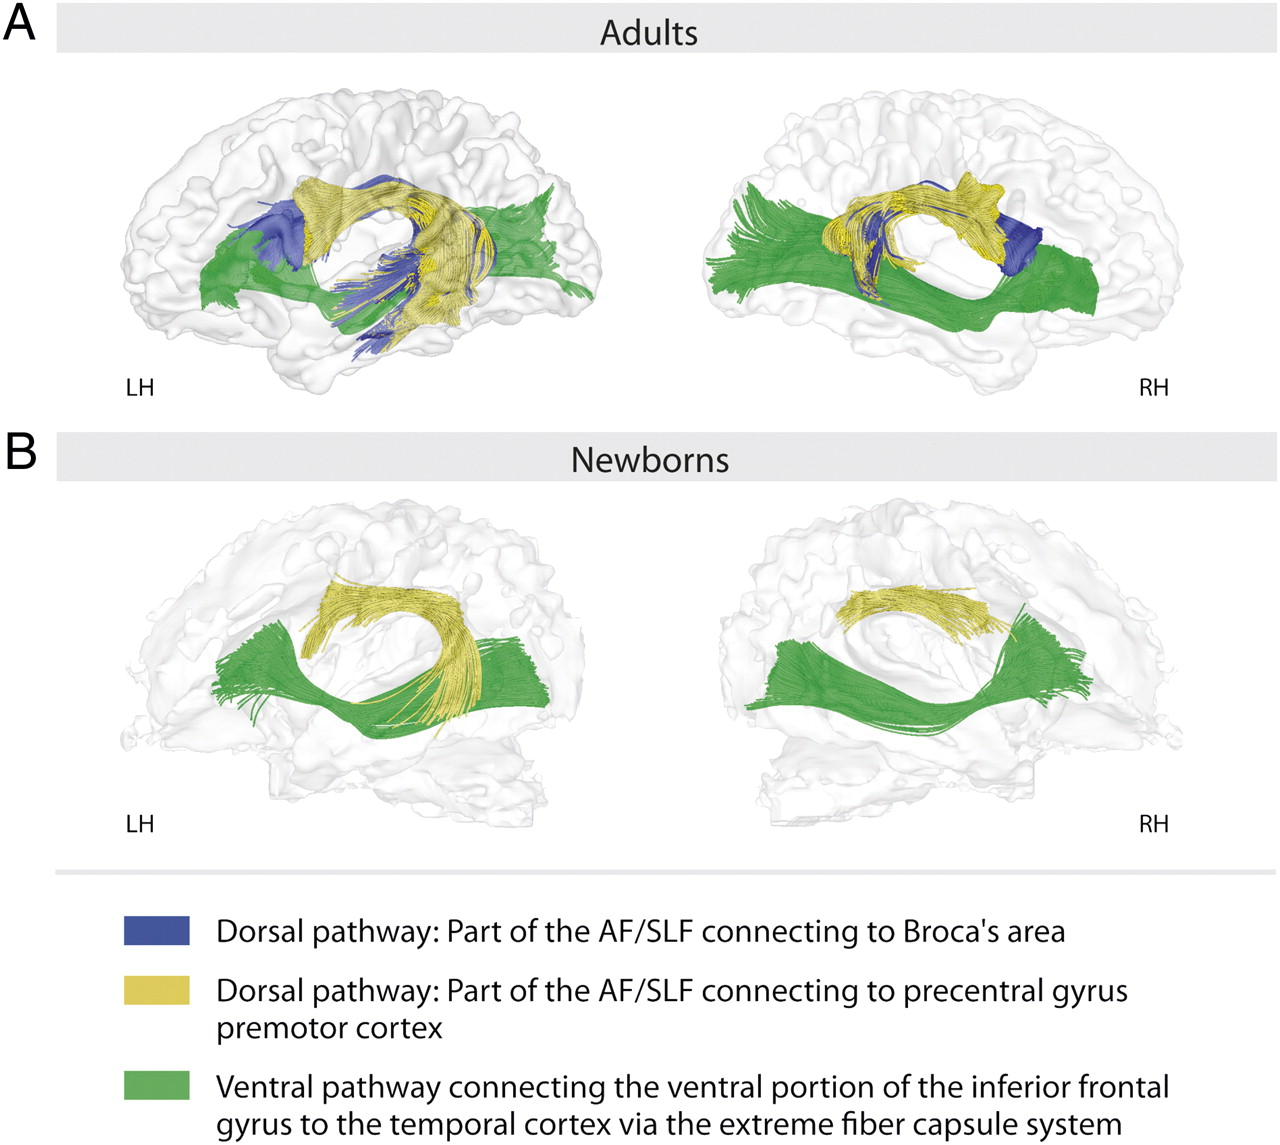
\includegraphics[width=1\textwidth]{Perani(2011)3}
	\caption[Perani(2011)3]{Perani(2011)对比了婴儿和成人听觉中枢的情况,发现婴儿颞叶到额叶见的联系只是初步建立,还不完善,由此推断新生儿只是听声音,但并不明白其含义.}
	\labfig{Perani(2011)3}
\end{figure}

上面这个系列实验是在实验室中通过严格的控制得出的结论,事实上,并不是只有在实验室中的实验才是科学实验,重要的是科学研究的思想。我们先简要说说\textbf{科学研究的思想},随后看看非实验室的研究可以怎样的出科学的结论.

\subsection{科学研究的思想与目标}

\begin{description}
    \item[1.系统的理论框架]
    只有有了系统的理论支持,收集数据才不是盲目的,上述实验中如果不是有Chomsky的理论支持,我们不会新生儿的语言获得情况有所兴趣,如果不是因为有FMRI研究技术的发展,我们不会想到用多功能核磁对新生儿进行研究.毕竟,一个刚出生两天的小婴儿,要其主观报告或者用其行为指标来反应其是否对语言有反应是不可能的.研究不是没有目的收集数据,而是有一定的理论支持,有一定的研究目的;
    \item[2.控制机制]
    主要是说的对无关变量进行控制,这一点和第三条一起说比较方便;
    \item[3.对象之间的因果关系]
    因果关系是心理学研究中最想得到的,想要做到为点需要有严格的控制.最理想的情况是研究者操控自变量在不同水平,并且控制无关变量,再对因变量进行观测,这样获得因变量观测值的差异就是由研究者在实验中让被试产生的,就可以很肯定的说是由自变量的变化导致的.关于这点我们还要再以后自变量的分类上谈,但此处要留个印象:最严格的因果关系是建立在实验中研究者人为造成的使被试形成的差异,比如上实验中输入的语料类型让婴儿由研究者的操作而导致的它们语言加工产生差异,这种差异是在实验室内产生的,是研究者明明白白控制了的,动因明确的.有些被试间的差异不是由研究者引起的,造成这个差异的原因也千奇百怪不得已而知,因此这类自变量往往不能得出严格的因果关系,比如说性别.因为行为学实验个体差异的关系,因此研究者通常用被试内设计,也就是一个被试要接受所有的处理,这样可以有效分离出被试间个体差异,这点我们后面要细谈,此处提及只是因为上实验(Peranti,2011)用的就是被试内实验设计,每个婴儿都听了这三段音频.
\end{description}


接下来我们以“对儿童说谎行为的研究”谈谈\textbf{科学研究目标}:

\begin{description}
    \item[1.描述]:如观察儿童说谎行为的各种不同表现形式、说谎的频率;
    \item[2.理解]:了解儿童说谎的原因(是否为了逃避批评或惩罚、或者为了获得某种利益?).我们知道儿童想要说谎必须有一定的认知机制,说谎不是一个简单的事情, 要有一定的认知能力才能说谎.要知道别人对问题是怎么想的,考虑别人怎么看问题才能说出来看起来比较严密的谎言,认知能力还没成熟的孩子说的谎在成年人看起来往往是可笑的;
    \item[3.预测]:什么样的家庭或学校环境下,什么年龄儿童可能出现说谎行为;
    \item[4.控制]:如果已经知道孩子在青春期喜欢说谎,并且这个现象不利于孩子的发展,那是否可以有合理的控制机制让说谎情况降到最低呢?
\end{description}


\subsection{心理学研究的途径}

下一步,我们继续讨论\textbf{心理学研究的途径},此处不会详细论述某种研究手段,想向各位传达的信息是,不是只有典型的实验研究才是研究,别的研究手段尽管没有对实验条件进行严格的控制,但这些手段都是科学的,都是为了一定的研究目的服务,也会进一步深入问题提供一个基础.额外想提醒的是,研究手段和研究目的紧密相关,有些现象没法用实验的手段,这点我们也放到后面的实验设计中谈.

\textbf{1.观察}

观察法指的是在自然状况下收集数据,描述某种现象包括自然现象,包括自然观察,问卷调查,个案研究.前面我们提到了儿童一岁半左右一个很有趣的词汇暴增现象——\textbf{词汇爆炸(vocabulary spurt)}.Bloom(1985)首先在国外儿童中发现了这个现象,那么中国儿童是否也存在这个现象呢?这就有赖于对汉语母语儿童的观察,我国学者确实发现在汉语母语儿童身上也发现了相同的现象(Li, 2007),下面介绍一下他们的研究.我们没法对6-7个月的儿童进行控制,让他们主观报告自己会说的词汇,因此只能让家长填写词汇问卷,判断哪些词是自己孩子说过的.这个词表数目还挺多的,让一个家长做完整个词表会造成较大的疲劳效应,因此实验中也匹配了一些“平行家长”,不过这都是控制机制,在此我不打算具体介绍.总之,在\reffig{Li(2007)}中我们确实看到,在18个月左右时,确实存在一个词汇量剧增的时间点.

这个实验中,我们不是被动的收集数据,而是有着某种特殊目的收集儿童的词汇量,并且这个实验结果得到了一个漂亮的结果.可见,描述性实验也失为一种有用的科学实验

\begin{figure}
    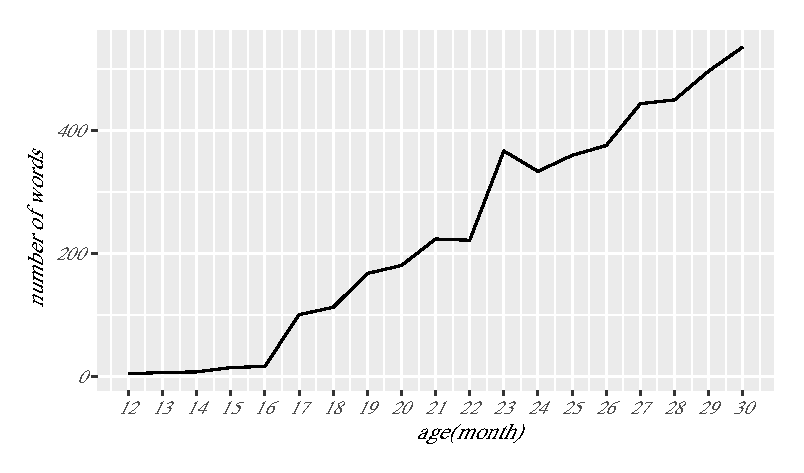
\includegraphics[width=0.8\textwidth]{Li(2007)}
    \caption{Li(2007)对12到30个月的汉语母语儿童进行了词汇量的追踪,结果发现了他们身上也存在词汇爆炸(vocabulary spurt)现象}
    \labfig{Li(2007)}
\end{figure}

\textbf{2.相关研究}
相关研究对两种现象(变量)之间的关系感兴趣,例如:吸烟与肺癌之间的关系.但是没法指因两个变量间引起与被引起的方向(到底吸烟引起肺癌,还是有肺癌基因的人倾向于吸烟不能从显著的相关中推论)

在对儿童语言发展的研究中,我们感兴趣的是孩子抚养人(特别是母亲)的语言使用清空对孩子会有什么样的影响,具体来说,父母寡言是否孩子也会寡言?父母受教育程度高是否导致孩子更喜欢说话?处于伦理道德的限制,我们只能记录孩子和父母的情况,不能对上述两个因素进行严格控制.

这个问题一直不能好好解决,因为要对一段录音中词语数进行统计是相当困难、工作量巨大的事情.不过LENA技术的出现让这种困境得以摆脱.这个程序可以识别婴儿的声音中的语言成分,并把一些非言语部分分离出去,比如哭声、吃东西的声音;它还可以分辨不同人的声音,这样也可以家长的说话情况.

这个实验的结果如\reffig{LENA}所示,我们能非常清楚地看到,父母地寡言和多言确实影响了孩子的与发展,
 
\begin{figure*}
    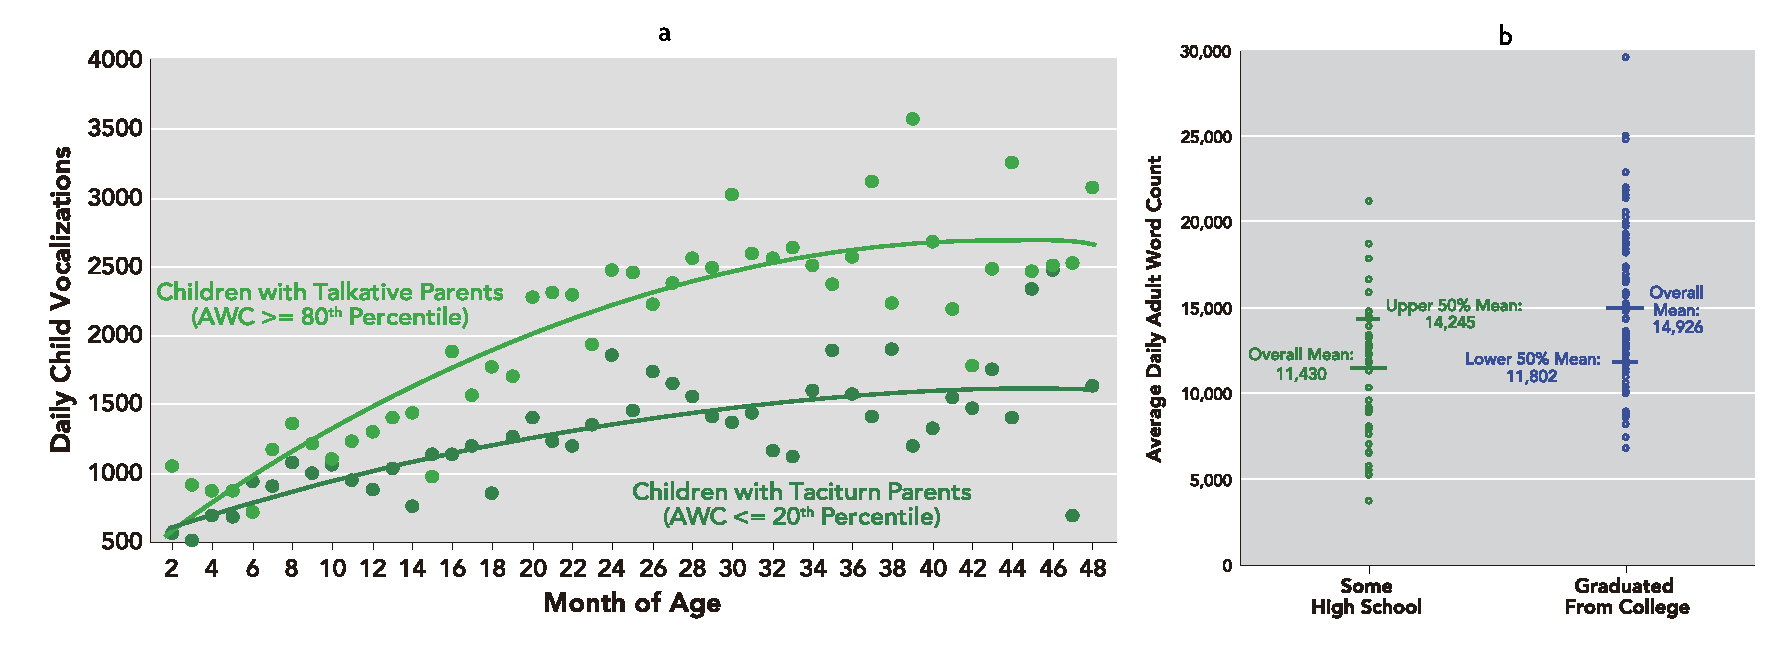
\includegraphics{LENA}
    \caption{用LENA研究父母多言寡言与受教育程度与孩子语言发展情况,结果发现这二者都和孩子的词汇发展成正相关}
    \labfig{LENA}
\end{figure*} 
 
\textbf{3.实验研究}

以Hagoort(2004)的一个研究为例看看他精细的设计.我们已经知道语义违反\sidenote{语义违反(semantic violation),指的是合乎语法要求却不符合词语的意义,如“这本书很咸”,从句法来看这句话是正确的,但是“咸”这个形容词不能修饰不是食物的名词,因此此处属于语义违反句子}会引起N400.还有一类句子错误,虽然语法、语义上都是正确的,但是和我们关于这个世界的认识是相违背的,比如“中国国家主席是位女士”.上述的两类错误涉及两种句子理解过程,一个是语义理解,一个是世界知识理解,以往人们认为这是两个独立的过程.Hagoort指出实际上这两种过程的区别不太好分开,因为很多词语都是不止有一个意思,多义词在特定语境中是什么意思要用世界知识来判断,进而Hagoort判断,世界知识违反(world knowledge violation)也会引起N400.

\begin{marginfigure}
    
\includegraphics{dutch_train}
    \caption{荷兰火车的配色,实际上的车型并非如此}
    \labfig{dutch_train}
\end{marginfigure}

实验的材料(见\reffig{Hagoort(2004)}中的文字)经过了精心的设计,Hagoort给世界知识违反、语义违反、正确句子下了三个操作定义,这里用了一个非常有意思的操作定义来表示世界知识违反:实验的被试都是荷兰人,荷兰的火车都是黄色为主色调的(配色类似\reffig{dutch_train}),因此“The dutch trans are white”显然不符合荷兰人心中存在的对火车的知识.结果非常证实了Hagoort的猜想,在\reffig{Hagoort(2004)}可以清楚地看到,正确句子没有引起N400,而语义违反和世界知识违反都引起了N400.

\begin{kaobox}[frametitle=问题:如果这个实验只保留世界知识违反和正常条件,可行吗?]
如果顺着这个实验的结果来推理,这么做是看起来是可行的:把这个实验结果上的语义违反条件去掉,世界知识违反也确实引起了N400.但是要注意,实验前研究者并不知道结果是什么.也就是说实验前的假设是:\\
(1)若世界知识违反可以引发N400,说明语义理解与世界知识理解是一个连续的过程;\\
(2)若世界知识违反没有引发N400,说明语义理解与世界知识违反是两个独立的过程.\\
如果没有语义违反条件,(1)的结论还是可以得出,但是(2)中似乎存在了点问题.因为实验结果不显著不一定是处理效应不存在,还可能是检验力低的问题.对于心理学实验,它的处理效应本身就不高,那些不太明显但是确确实实存在的现象才有研究和发掘的价值.因此处理效应的显著需要较高检验力,实验设计一定要尽力精准和敏感.但不是所有实验都可以做到那么精准,想要得到漂亮的结果不是一件容易的事.在本实验中,如果没有语义违反做对照,在世界知识违反不显著时,研究者没法区分这是由实验不敏感导至的,还是由处理效应不存在导致的.因为语义违反已经被无数实验证明一定会引起N400,所以加上语义违反这个条件,就可以对实验的敏感性进行检验.这样(2)就可以拆分为以下两个假设:\\
(1)若世界知识违反没有引起N400,语义违反没有引起N400,则说明实验不够敏感,需要重新设计实验,处理效应是否存在有待继续检验;\\
(2)若世界知识违反没有引起N400,语义违反引起N400,则说明世界知识范围确实不会引起N400,世界知识违反和语义违反是两个独立的过程.
\end{kaobox}

\begin{figure}
    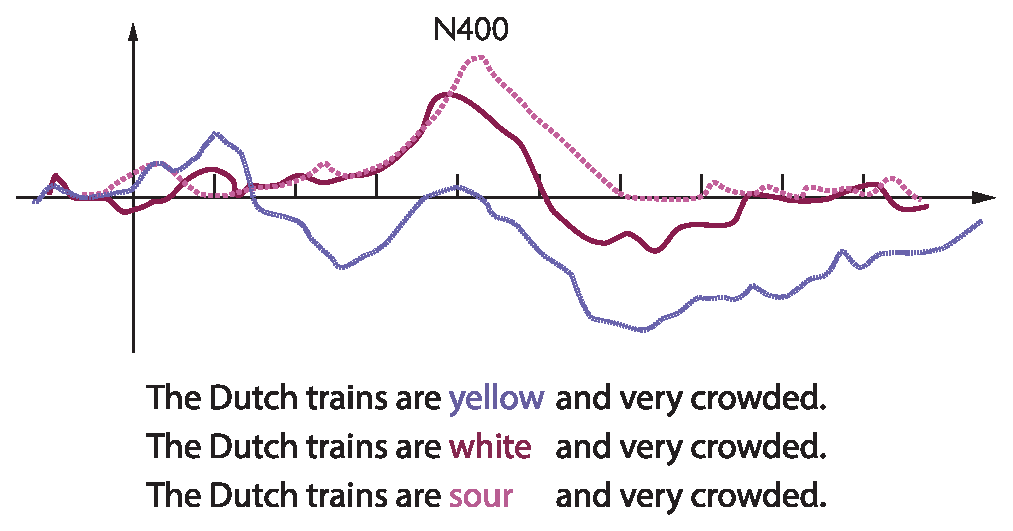
\includegraphics[width=1\textwidth]{Hagoort(2004)}
    \caption[Hagoort(2004)]{Hagoort(2004)给被试看三个句子并记录其脑电,发现世界知识违反的句子也会引起N400,进而说明了语义理解与世界知识理解是一个整体而不可以分割的过程.}
    \labfig{Hagoort(2004)}
\end{figure}

分析一下这个实验为什么是一个好实验.首先在自变量研究者控制了关键词的不同,在无关变量的控制上,除了关键词以外的句子都一摸一样,这样就排除了由于文字本身难度、熟悉度、使用频率带来的无关变异.实验设计上,采用被试内实验设计,每个被试都读了这三个句子,控制了所有的被试间的差异.这样总得来看,操作定义下得很精准、无关变量控制得也很巧妙,是一个值得我们学习的非常典型的实验设计.